\item \textbf{Augmented Reality for Enhanced Interaction and Safety}
   % Augmented reality user interface design and experimental evaluation for human-robot collaborative assembly - reference : CHU2023313
    % Leveraging \ac{AR} can significantly improve the interaction between humans and robots by providing intuitive visualizations and reducing the need 
    % for continuous visual contact. As demonstrated by Chu et al. \cite{CHU2023313}, effectively conveying robot intentions through \ac{AR} visuals enhances 
    % worker awareness of their surroundings, thereby improving safety and efficiency in collaborative tasks. 
    
    % After analysing previous related work and implemented methodologies, 

    % The \ac{AR} interfaces clearly visualize the 
    % robot's work envelope, as depicted in Figure~\ref{fig:ar-envelope}, enabling human operators to navigate shared workspaces safely and efficiently.
    
    % \begin{figure}[htp]
    %     \centering
    %     \begin{subfigure}{.5\textwidth}
    %         \centering
    %         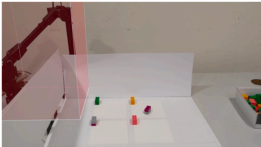
\includegraphics[width=0.9\linewidth]{figs/a-work-env.png}
    %         \caption{}
    %         \label{fig:sfig1}
    %     \end{subfigure}%
    %     \begin{subfigure}{.5\textwidth}
    %         \centering
    %         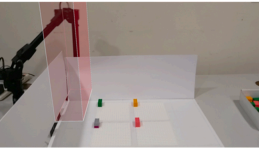
\includegraphics[width=0.9\linewidth]{figs/b-work-env.png}
    %         \caption{}
    %         \label{fig:sfig2}
    %     \end{subfigure}
    %     \begin{subfigure}{.5\textwidth}
    %         \centering
    %         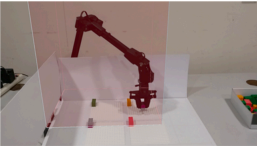
\includegraphics[width=0.9\linewidth]{figs/c-work-env.png}
    %         \caption{}
    %         \label{fig:sfig3}
    %     \end{subfigure}%
    %     \begin{subfigure}{.5\textwidth}
    %         \centering
    %         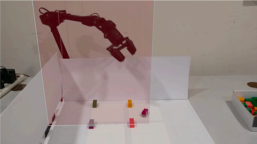
\includegraphics[width=0.9\linewidth]{figs/d-work-env.png}
    %         \caption{}
    %         \label{fig:sfig4}
    %     \end{subfigure}
    %     \caption{AR displayed work envelope of robotic arm \cite{CHU2023313}}
    %     \label{fig:ar-envelope}
    % \end{figure}
    

%     %notas para adicionar sobre o artigo - acima - 
%     The experiment aims to verify and
%     cross-compare the effectiveness of visual and haptic cues in various forms that convey the robot intent to human.
%     Analysis of the work performance and gazing behavior of participants shows that both cues can reduce their
%     visual attention on the moving robot during the collaboration. 
%     [10] emphasized the importance of human information
%     communication on assuring safety in HRC. They considered AR as an
%     ideal interface that enables the human and robot to ground their
%     communication and intentions by sharing an ego-centric view. AR also
%     allows for an exocentric view of the collaborative workspace that provides spatial awareness. This study suggested that a human-robot
%     collaborative system based on multimodal interactions would be more
%     effective and natural than unimodal.
%     Since  AR headsets still have a very limited field of view compared to the human vision. Visual guidance for localizing out-of-view objects in the limited display space often causes visual conflicts such as cluttering or occlusion of information [11]
%     Other works [12] proposed a visualization interface in AR HMD that superimposed the intended robot motion onto the user’s
%     view of real environment verifying that  the user determined where the robot was going to move using the interface more
%     quickly and accurately than 2D display or no assisted visualization.

%     the article itself outlines that providing AR user interfaces with either visual, haptic or multi-modal cues for HRC are benefitial.
%         Visual-based AR (cues) help overcome limitations arising from complex environments by superimposing visuals in an HMD without compromising robot mobility. this system also revealed to reduce the idle robot time as well as the task completion time when compared to the baseline without the user interface or the space sharing. However, user experience assessment showed that the HoloLens setup was not yet technically mature on the shop floor, particularly the limited field of view.
%         Visual feedback on a screen displayed the swept volume generated by the planned robot trajectory. Experimental data indicated that the human
%         workers felt more comfortable and had a better understanding of the robot motion and goals using multi-modal feedback. 
%         Haptic cues - It is sometimes advantageous in industrial environments over visual and auditory modalities, which could be overloaded or blocked on site. Vibrotactile devices have been applied to control industrial robot and to inform users of approaching singularities and joint limits in a factory [22]
%         Visual and acustic - aimed to reduce human's anxiety related to the unpredictability of the robot motion in a shared workspace. Acoustic feedback was used to alert the human when the robot had detected a possible collision and changed the planned motion.

%         % \ac{ROS} was useful, said by this article, this reinforces that the model i developed goes in line to what the literature supports
%         Implementing the system using the Robot Operating System also allowed modularity and extendibility for such a multi-device and multi-user approach.

%         % see conclusion - were the visual and haptic cues that communicated the robot motion useful in a collaborative assembly for the user?

%         % experiment:
%         During the assembly, a human operator picks, fetches, and stacks LEGO blocks onto specific work areas determined by the block color, while a desktop robot transports extra blocks to the areas over a wall.

%         In addition, both visual and tactile cues are presented in two forms that convey the robot motion with different degrees of information in AR.

%         % display 
%         As shown in figure \ref{f:area-1}, the operator was collaborating with a robot arm in a 25 cm × 25 cm work space in the middle of the table. The space was divided into four areas and each held LOGO blocks of a different color (see Fig. 2). The robot arm was mounted outside of the work space separated by a wall.

%         \begin{figure}[!htpb]
%             \centering
%             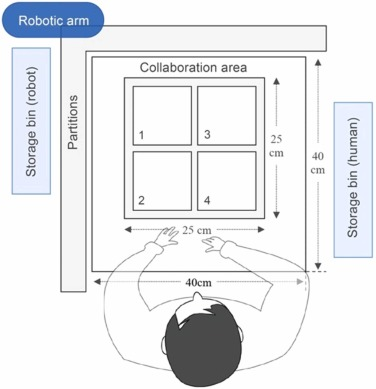
\includegraphics[width=0.4\linewidth]{figs/area-1.jpg}
%             \caption{Collaborative work space in the experiment, \cite{CHU2023313}}
%             \label{f:area-1}
%         \end{figure}

%         The space was divided into four areas and each held LOGO blocks of a different color (see figure \ref{f:robot-area-1}). The robot arm was mounted outside of the work space separated by a wall.

%         \begin{figure}[!htpb]
%             \centering
%             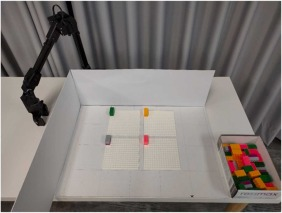
\includegraphics[width=0.4\linewidth]{figs/robot-area-1.jpg}
%             \caption{Actual work environment in the experiment, \cite{CHU2023313}}
%             \label{f:robot-area-1}
%         \end{figure}

%         The human and the robot independently performed individual tasks without a physical contact during the experiment. The operator picked up a block randomly from a storage bin on the right; then assembled the block into the area corresponding to its color. The storage bin contained 12 blocks of each different color. In contrast, the robot picked up a block at random times from the storage area on the left, which contained 4 blocks of each color. It then delivered the block to one of the four areas, also at random. The manual assembly of LEGO blocks must comply with the
%         following instructions. First, only one block was assembled at one time.
%         The operator could finish the assembly by using one or both hands.
%         Second, a block must be assembled to the area matching its color. The
%         block assembly started from the upper left of each area; then sequentially progressed from left to right and from up to bottom. Next, a block
%         could not be placed on top of existing blocks. The operator was asked to
%         complete the tasks as efficient as possible, while avoiding any collision
%         or physical contact with the robot.

% % visual and haptic user implemented interfaces
%         The visual interface was implemented in the HoloLens 2, which displayed the robot’s planned motion and the swept volume generated by the robot trajectory. The visual interface was designed to provide the operator with a clear understanding of the robot’s intended motion and goals. The haptic interface was implemented using the SenseGlove Nova™, which provided force feedback to the operator’s hand. The haptic interface was designed to alert the operator of the robot’s planned motion and to guide the operator’s hand to the correct assembly location. they can be seen in the figure \ref{fig:haptic-visual-cues}.

%         \begin{figure}[htp]
%             \centering
%             \begin{subfigure}{.5\textwidth}
%                 \centering
%                 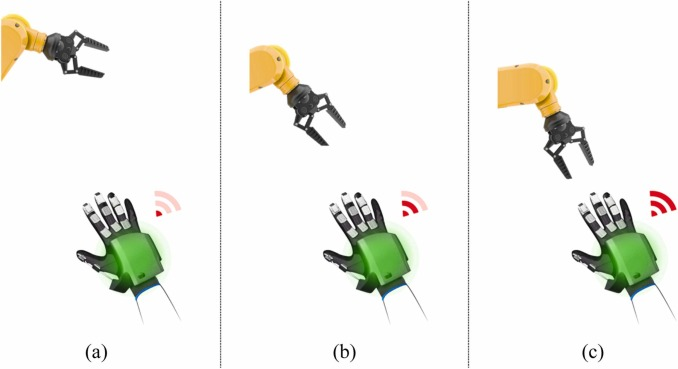
\includegraphics[width=0.9\linewidth]{figs/haptic-cues.jpg}
%                 \caption{Indicating the gripper’s destination using vibration on different human fingers.}
%                 \label{fig:sfig1}
%             \end{subfigure}%
%             \begin{subfigure}{.5\textwidth}
%                 \centering
%                 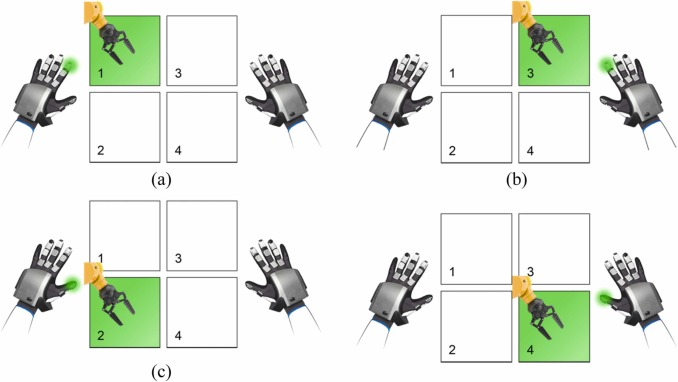
\includegraphics[width=0.9\linewidth]{figs/visual-cues.jpg}
%                 \caption{Indicating the proximity of gripper via change of vibration frequency.}
%                 \label{fig:sfig2}
%             \end{subfigure}
%             \label{fig:haptic-visual-cues}
%         \end{figure}
        

%         % AR interfaces - integration:
%         A WidowX 250 Robot Arm developed by Trossen Robotics was used
% in the experiment. This device is a 5-DOF desktop robotic arm with a
% 650-mm work range centered at the base. The robot
% control is realized by a computer through the Robot Operating System
% (\ac{ROS}) [42]. \ac{ROS} supports the motion planning framework MoveIt [43],
% which provides fundamental open-source functions for robot motion
% planning and manipulation. (this part is similar to the one of the project i am working with- robot with \ac{ROS} and also Moveit integrated - useful to mention)
% the manual tasks were performed while wearing a Microsoft HoloLens 2: The two visual interfaces were mainly implemented in HoloLens 2.
% We adopted SenseGlove Nova™, shown in figure \ref{f:HTC-gloves} to produce force feedback required
% by the haptic user interfaces. It is a programmable device commonly
% used in \ac{VR} applications to simulate tactile perception for
% high interactivity. To integrate the device with AR applications involves
% recognition of the user’s hand gesture and position in real environment.
% For this purpose, a HTC VIVE tracker was attached on each glove.

% \begin{figure}[!htpb]
%     \centering
%     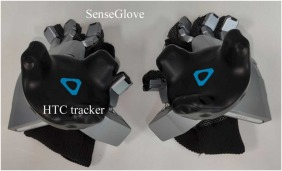
\includegraphics[width=0.6\linewidth]{figs/gloves.jpg}
%     \caption{Attaching HTC trackers on SenseGlove, \cite{CHU2023313}}
%     \label{f:HTC-gloves}
% \end{figure}

% Figure \ref{f:system-framework} shows the system framework proposed to integrate hardware
% devices with the UNITY engine residing on a desktop computer as an
% application server. The computer connected with the robot arm using a
% USB cable via Ubuntu v20.4 and executed motion control in \ac{ROS}. It
% communicated with the HoloLens 2 and SenseGlove using WiFi and
% Bluetooth, respectively.

% \begin{figure}[!htpb]
%     \centering
%     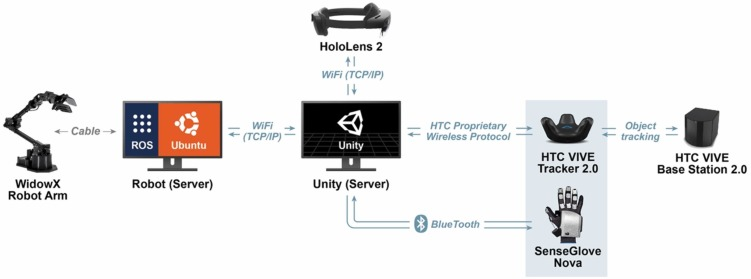
\includegraphics[width=0.6\linewidth]{figs/system-framework.jpg}
%     \caption{The system framework for integration of hardware devices in the experiment, \cite{CHU2023313}}
%     \label{f:system-framework}
% \end{figure}

% Section: Implementing AR and Digital Twins in Human-Robot Collaboration (HRC)

\paragraph{\textbf{Experiment Design: Collaborative LEGO Assembly Task}}
    The experimental setup involved a human operator collaborating with a desktop robotic arm in a 25 cm × 25 cm workspace. The operator's task was to pick, fetch, and stack LEGO blocks onto specific areas of the workspace, sorted by color, while the robot arm delivered extra blocks randomly into the workspace over a wall. It aimed to verify and cross-compare the effectiveness of visual and haptic cues in conveying the robot’s intent to the human operator. Figures \ref{f:area-1} and \ref{f:robot-area-1} depict the collaborative workspace and robot setup.

    \begin{figure}[!htpb]
        \centering
        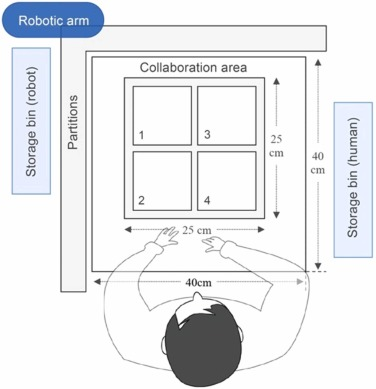
\includegraphics[width=0.4\linewidth]{figs/area-1.jpg}
        \caption{Collaborative work space in the experiment \cite{CHU2023313}}
        \label{f:area-1}
    \end{figure}

    \begin{figure}[!htpb]
        \centering
        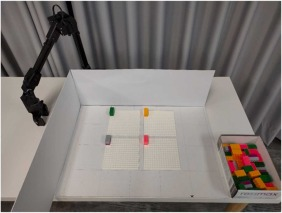
\includegraphics[width=0.4\linewidth]{figs/robot-area-1.jpg}
        \caption{Actual work environment in the experiment \cite{CHU2023313}}
        \label{f:robot-area-1}
    \end{figure}

    \paragraph{\textbf{System Framework}}
    UNITY engine running on a desktop computer allowed to communicat with the robot and the \ac{AR} devices. As shown in figure \ref{f:system-framework}, the system's architecture used USB connections and WiFi/Bluetooth for communication between the HoloLens, SenseGlove, and Robot. A HTC VIVE tracker was attached to the gloves to track the user's hand movements, providing haptic feedback in synchronization with the \ac{AR} visuals.

% remove this figure (done) - change the above text to reflect the removal of the figure
    % \begin{figure}[!htpb]
    %     \centering
    %     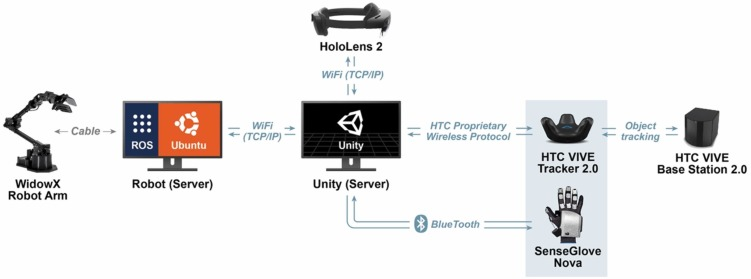
\includegraphics[width=0.75\linewidth]{figs/system-framework.jpg}
    %     \caption{The system framework for integration of hardware devices in the experiment \cite{CHU2023313}}
    %     \label{f:system-framework}
    % \end{figure}

    The framework allowed seamless interaction between the physical and virtual worlds, enabling real-time feedback for the operator, thus improving decision-making and task efficiency in the assembly process.



    % \paragraph{Conclusion}
    % The experiment with LEGO assembly and the integration of \ac{AR} and haptic feedback showed that visual and haptic \ac{AR} interfaces effectively communicate robot motion intent, improving interaction and collaboration. The system, using \ac{ROS} and MoveIt, provided a flexible and scalable platform for HRC in a shared workspace. The findings of this study align well with current literature, which emphasizes the importance of multimodal feedback in enhancing human-robot interaction in smart manufacturing.

%  parece-me que a parte de cima parece estar bem estruturada e revelar as vantagens do artigo explorado - ver as referencias que faltam e organizar melhor a estrutura e as figuras - remover depois o texto comentado que está acima de toda esta parte que escrevi agora - 24 set 01h56

    %verificar este artigo e mencionar coisas mais úteis, isto está mto breve
    % Additionally, Lotsaris et al.~\cite{LOTSARIS2021301} presented an \ac{AR} application that facilitates operator work in human-robot environments by 
    % enabling coexistence and improving communication. Their system displays safety fields around the robot using different colors to represent safe and 
    % dangerous regions, enhancing situational awareness and reducing the risk of accidents. However, a significant challenge remains in the complexity of
    % recognizing detailed information through haptic feedback, indicating a need for more sophisticated algorithms and sensors to capture and translate 
    % complex robot actions into intuitive \ac{AR} visualizations.
    


%%%%%%%%%%%%%%%%%%%%%%%%%%%%% 24 set - 17h - deixar ??? ver o que este artigo diz e se é relevante
    % \item \textbf{Virtual and Augmented Reality for Intuitive Robot Programming}
    
    % Programming robots using Virtual Reality (VR) and \ac{DT} introduces innovative methods that capture human movements, reducing the learning curve for 
    % non-experts and enabling intuitive programming of complex tasks. Bolano et al.~\cite{Bolano2020} demonstrated that bilateral communication between 
    % the VR environment and the robot’s hardware allows changes to be made in both the virtual and physical systems. This full immersive experience 
    % enables users to interact directly with the robot's end effector through holographic interfaces, facilitating the selection and application of 
    % desired operations seamlessly.
    
    % Similarly, Burghardt et al.~\cite{burghardt2020programming} explored programming DTs using VR, where the robot reproduces human movements within a virtual 
    % environment. This approach ensures that the robot can accurately mimic complex human actions, which is particularly beneficial in tasks that are 
    % challenging to automate traditionally. The integration of Unity and \ac{ROS} platforms further enhances the functionality by 
    % providing robust communication and real-time data processing capabilities.
    
    % In the context of mobile platforms, Lotsaris et al.~\cite{LOTSARIS2021301} highlighted the challenges of achieving friendly interaction in shared 
    % working environments due to the absence of effective communication between operators and robots. Their AR application addresses this by displaying 
    % safety fields and facilitating better communication, thereby improving the overall interaction experience.
    
    % \begin{figure}[h]
    %     \centering
    %     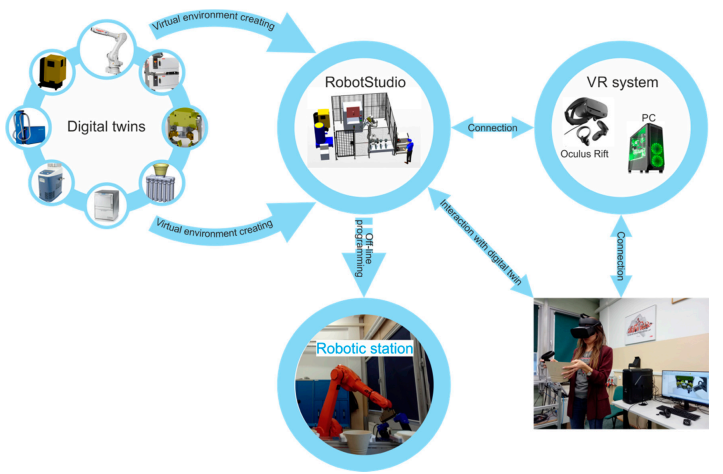
\includegraphics[width=0.9\linewidth]{figs/vr-oculos-dt.png}
    %     \caption{Schematic diagram of the building and programming of a robotic station alongside VR technologies \cite{burghardt2020programming}}
    %     \label{fig:vr-oculos-dt}
    % \end{figure}
    
    % Despite these advancements, challenges such as the need for high precision in replicating human movements and the complexity of \ac{VR} tracking 
    % technology persist. Improvements in algorithms, particularly those utilizing Machine Learning (\ac{ML}) techniques, are essential to ensure that 
    % robotic movements closely mimic human operators' actions \cite{Burghardt2020}.
    

    % % 
% \subsubsection{Digital Twins in Academia and Industry}

% Digital Twins (DT) have gained significant traction in both academic research and industrial applications in recent years. Despite their growing prominence,
% there is no universally accepted formal definition of a DT. 

% Nevertheless, the majority of reputable researchers concur that a DT is a \ac{CPS} comprising at
% least three essential components: 
% \begin{itemize}
%     \item A physical system,
%     \item A virtual model,
%     \item Connections facilitating bidirectional communication between the physical and virtual models \cite{TaoFei, 8477101, ROSEN2015567}.
%     % confirm these citations above
% \end{itemize}

% In academic settings, DTs have been explored across a wide array of applications, including machine tool life management, product health management,
% smart cities, and patient health monitoring, among others \cite{8361285, TAO2018169, isprs-archives-XLII-4-W7-37-2017, 10.1007/978-3-030-23162-0_19, 6296978}. These applications demonstrate the versatility and potential of DTs in enhancing efficiency, predictive maintenance, and system optimization. 
% % confirm these citations above

% In the industrial sector, numerous companies, such as Siemens, offer software and platform solutions aimed at creating DTs for their industrial partners. 
% However, some critics argue that these solutions represent digital shadows rather than true DTs. 

% The primary contention is the lack of bidirectional communication capabilities, specifically, while changes in the physical system can influence the virtual model, the reverse—where modifications in the virtual model impact the physical system—is often absent \cite{CIMINO2019103130}. 

% Figure \ref{f:dt-structure}, \cite{dt_model} outlines the \ac{DT} reference model, illustrating the bidirectional communication between the physical 
% and digital entities. This configuration underscores the distinction between true DTs and digital shadows, the latter often criticized for lacking 
% interactive communication capabilities \cite{CIMINO2019103130}.



% % However, the concept of \ac{DT} lacks a standardized definition, leading to a variability in the scope and execution of \ac{DT} implementations. 
% % The dual nature of cyber and physical components in \ac{DT} makes \ac{AR} a suitable companion for visualizing and interacting with these complex 
% % systems (cite the article itself).

% As emphasized by Liu et al.~, "A true DT must include bidirectional communication instead of having a virtual model that updates
% according to a physical system." 
% Given that the concept of \ac{DT} lacks a standardized definition, leading to a variability in the scope and execution of \ac{DT} implementations and
% defining a misconception, the critical distinction between three types of interaction is further ilustrated in Table ~\ref{tab:levels_of_control}, ~\cite{liu2022state}.
% % This critical distinction is further illustrated in Table~\ref{tab:levels_of_control}.




\subsubsection{Integration of Augmented Reality with Digital Twins} % verify this section references - if it matches what it said - 23 set 19h56

Integration \ac{AR} with \ac{DT} technology represents a significant advancement in enhancing user interactions with complex systems. 
\ac{AR} overlays virtual data directly onto physical objects, thereby providing a more intuitive and engaging interface for users. 
This capability is particularly beneficial in industrial settings where \ac{AR} can facilitate more efficient and effective operation and 
maintenance processes \cite{article12, peddie2017augmented}.

Despite the numerous advantages of \ac{DT}s, a significant challenge lies in the effective visualization of the complex data they generate. 
As interest in \ac{DT}s grows, it becomes increasingly important to provide users with intuitive and accessible methods to interpret and interact 
with this data. According to \cite{article12}, the benefits of real-time data and information provided by \ac{DT}s cannot be fully realized without 
proper visualization techniques that present complex information in a clear and uncluttered manner, especially for users with limited technical expertise.

\ac{AR} offers a promising solution to this challenge by enhancing data visualization and user interaction. Traditionally, users interact with digital 
information through 2D interfaces such as screens and monitors. However, \ac{AR} expands this interaction into the real world by overlaying virtual 
data onto physical objects, creating immersive 3D experiences that align with users' familiar environments \cite{peddie2017augmented}. This 3D visualization enables
users to better understand and absorb information through visual cues, which are often more effective than textual or auditory information \cite{article-teaching}.
For instance, projecting maintenance instructions directly onto a machine allows users to perform maintenance tasks more efficiently compared to 
consulting physical manuals \cite{inproceedings}. Moreover, \ac{AR} has been successfully utilized in various manufacturing processes to provide guidance 
for maintenance procedures and to train novice workers, demonstrating its versatility and effectiveness in industrial settings \cite{ong2004virtual}.

By integrating \ac{DT} with \ac{AR}, it is possible to monitor the state of a system in real-time while simultaneously displaying relevant
data and information through \ac{AR} interfaces. This integration not only enhances the user experience but also improves operational efficiency and 
safety by providing actionable insights in an intuitive and accessible manner.




    In its presented work, Chu et al. (2023), reviewed several previous studies that gathered and exposed information on implementing \ac{AR} with \ac{DT}.Specifically, it integrates a real robot with visual and haptic \ac{AR} interfaces and explains their development \cite{CHU2023313}.
    
    \paragraph{\textbf{\ac{AR} and \ac{HRC} Integration}}
    Green et al. outline that \ac{AR} interfaces with visual, haptic, acoustic, or multi-modal cues are beneficial for \ac{HRC}. \ac{AR} is considered an ideal interface to enhance human-robot communication by providing both ego-centric (ability to share remote views) and exocentric (ability to visualize the robot relative to the task space) views of the collaborative workspace, improving spatial awareness and interaction \cite{doi:10.5772/5664}. 
    
    It has been demonstrated that multimodal interactions, such as audio-tactile feedback, can significantly enhance the \ac{HRC} experience by making it more intuitive and effective. These multimodal approaches provide valuable insights that would otherwise be limited, such as overcoming the restricted \ac{FOV} in \ac{HMDs}.
    % For instance, research has shown that while audio-tactile guidance might be slower compared to visual methods like EyeSee360, it offers a similar or even slightly better accuracy rate. 
    Moreover, it can be especially beneficial for users with visual impairments, as the same information is conveyed through another sensory channel without degrading performance.

    Visual \ac{AR} cues, implemented via \ac{HMDs}, allow users to navigate complex environments by overlaying visual information without hindering the robot’s movement. However, challenges like the limited \ac{FOV} of devices like the HoloLens present obstacles in industrial settings.
    In scenarios where visual and auditory modalities are overwhelmed, haptic feedback provides a viable alternative. Vibrotactile devices, for instance, have been successfully used to alert operators about robot motion, approaching singularities, and joint limits in factory environments. Acoustic feedback also helps reduce human anxiety in shared workspaces by warning users of potential collisions or sudden changes in the robot’s trajectory \cite{9199570}.

    In their study, Lasota et al. conducted a human subject experiment to evaluate both the objective and subjective impacts of human-aware motion planning. The experimental results demonstrated clear improvements in task performance and team fluency metrics. Specifically, participants working with a robot employing human-aware motion planning were able to complete collaborative tasks in less time, exhibit higher degrees of concurrent human-robot motion, and experience reduced idle times for both the human and the robot \cite{doi:10.1177/0018720814565188}. Additionally, these participants maintained greater separation distances, contributing to enhanced safety and reduced collision risk compared to interactions with a standard, non-adaptive robotic system.

    These results underscore the dual benefit of human-aware motion planning: not only does it improve the functional performance of \ac{HRC} by enhancing task efficiency, but it also significantly elevates the perceived safety and comfort of human collaborators, which are critical factors in reducing stress-related health risks in industrial or high-stakes environments.

    % Lasota~et.al, afirm that in a \ac{HRC} scenario where two distinct modes for robot operation were implemented, standard and human-aware, users reported feeling safer when the mode was able to differentiate between user actions and the surrounding environment. 

    \paragraph{\textbf{Implementation Techniques}}
    The system was developed using the \ac{ROS} to control a WidowX 250 Robot Arm, which provided the flexibility and modularity required for a multi-device and multi-user setup. MoveIt framework  was used for robot motion planning and manipulation, aligning with the technical model proposed in other robotics literature. The integration of \ac{ROS} reinforces the modularity and adaptability of the system, making it easier to manage \ac{HRC} in a shared environment.

    % \footnote{\url{https://moveit.ai/}, acessed in 2024-09-24}

    Both \ac{AR} and \ac{DT} models were implemented using a combination of hardware and software tools, like the Microsoft HoloLens 2 for the visual interfaces and a SenseGlove Nova™ which provided haptic feedback.
    Through the use of a HoloLens, the robot’s planned trajectory and swept volume were visually displayed, enabling the user to anticipate its actions. Simultaneously, the haptic interface provided vibration feedback to signal the robot’s proximity and intended target locations. As illustrated in figure \ref{fig:haptic-visual-cues}, these multimodal cues were presented in two distinct forms, each conveying varying levels of detail about the robot’s movement.

    \begin{figure}[htp]
        \centering
        \begin{subfigure}{.49\textwidth}
            \centering
            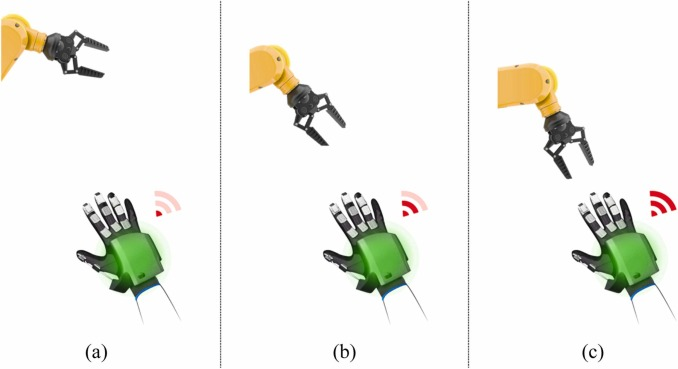
\includegraphics[width=0.9\linewidth]{figs/haptic-cues.jpg}
            \caption{Indicating the gripper’s destination using vibration on different human fingers.}
            \label{fig:sfig1}
        \end{subfigure}%
        \begin{subfigure}{.49\textwidth}
            \centering
            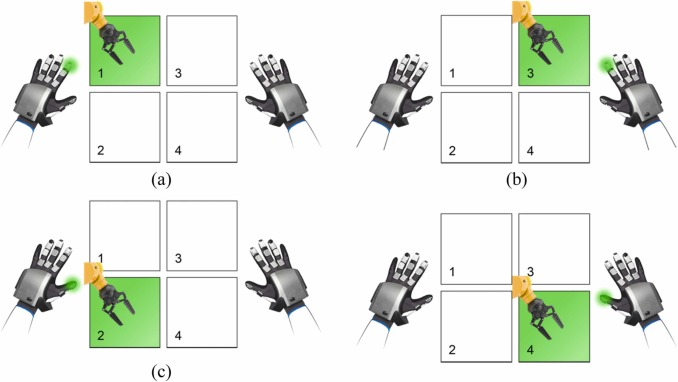
\includegraphics[width=0.9\linewidth]{figs/visual-cues.jpg}
            \caption{Indicating the proximity of gripper via change of vibration frequency.}
            \label{fig:sfig2}
        \end{subfigure}
        \caption{Visual and haptic interfaces used in the experiment \cite{CHU2023313}}
        \label{fig:haptic-visual-cues}
    \end{figure}


    The operator and robot worked independently, without physical contact, adhering to a sequence of tasks. While the operator picked up blocks randomly and placed them in the correct colored area, the robot randomly delivered blocks from the storage bin to one of the four workspaces. This task required careful coordination to avoid collision and optimize assembly efficiency, highlighting the benefits of \ac{AR}-based interfaces.

    \paragraph{\textbf{Advantages of Multimodal Cues}}
    The experiment demonstrated that using a combination of visual and haptic cues led to better task performance, as these cues helped the human operator predict the robot's movements, reduce visual strain, and enhance safety. The visual interfaces (especially those displaying proximity) outperformed others in usability, while haptic feedback was useful in environments where visual information might be insufficient or overloaded. Acoustic cues were also mentioned in the literature as a means to reduce anxiety in unpredictable robotic motions.

% 
\subsection{AR-Assisted Multi-Robot Systems for Enhanced Control and Coordination}

    % \item \textbf{}
    
    The use of \ac{AR} in real-time and planned control modes for multi-robot manufacturing systems significantly improves interaction, operational 
    safety, and efficiency. Li et al.~\cite{LI2022102321} demonstrated how operators can manage and coordinate multiple robots more effectively using 
    \ac{AR}-assisted DTs. Figure~\ref{fig:physical-digital} illustrates the dual view where users interact with the physical setup of two collaborating 
    robots and view their virtual counterparts via Microsoft Hololens \ac{AR} glasses. This immersive and intuitive control experience allows for 
    real-time simulation and monitoring of manufacturing processes and robot operations.
    
    \begin{figure}[!htpb]
        \centering
        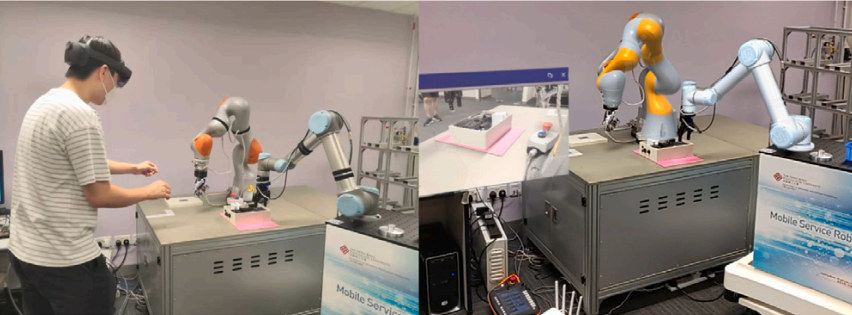
\includegraphics[width=0.85\linewidth]{figs/physical-digital.png}
        \caption{\ac{AR}-assisted \ac{DT}-enabled multi-robot collaborative manufacturing system \cite{LI2022102321}}
        \label{fig:physical-digital}
    \end{figure}

    Despite the promising advancements, issues such as \ac{DT} model accuracy and network latency continue to affect system performance. Future work must 
    focus on enhancing the fidelity and responsiveness of \ac{AR}-assisted \ac{DT} systems to fully realize their potential in industrial applications 
    \cite{LI2022102321}.

    Additionally, Ong et al.~\cite{ong2020} presented an AR-assisted robot programming system for welding applications. Their user-friendly interface 
    simplifies and accelerates the programming process by allowing users to define welding points and orientations using a handheld pointer. 
    The \ac{AR} interface enables users to validate programmed tasks within the real robot workspace, enhancing both accuracy and efficiency.
    
    Further advancements include the use of smart glasses and smartphones for robot manipulation. Malí et al.~\cite{7819154} developed an \ac{AR} 
    application that allows users to adjust robot axis values, highlight specific robot points with 3D arrows, navigate to invisible robot points using
    leading lines, and provide instructions via text and touch interactions. This system was evaluated in a production cell with an industrial robot, 
    demonstrating improved usability and interaction capabilities.

    Puljiz et al.~\cite{puljiz2019conceptsendtoendaugmentedreality,puljiz2} explored various AR-based methods for robotic arm programming using devices like Microsoft HoloLens. 
    Their approaches include hand-guided task programming, augmented trajectories, and the creation of spatial maps for waypoint placement and virtual 
    trajectory execution. These methods enable intuitive and precise programming of robotic arms, facilitating seamless integration of virtual instructions 
    with real-world robot operations.
    
    % analise do artigo - AR-assisted digital twin-enabled robot collaborative manufacturing system with human-in-the-loop - ref: LI2022102321
    In today's highly competitive market, manufacturing is evolving towards large-scale individualization and personalization, leading to an increased demand for flexibility and automation in manufacturing systems. To meet these personalization requirements, human operators are increasingly integrated into the production process~\cite{1}, collaborating with industrial robots that are well-developed and play a significant role in efficiently handling complex manufacturing tasks~\cite{2,3}.
    % rephrase this below sentence
    However, most existing robotic systems still carry out pre-programmed tasks in a routine manner with limited intelligence.

    To address this limitation, two effective human--robot collaborative alternatives have emerged. The first is robot learning, which aims to train robots by leveraging advanced \ac{AI} techniques~\cite{6}. The second, more pertinent to our interests, involves placing a human expert in-the-loop to teach or teleoperate the robot remotely.

    % reformulate this part
    % This second alternative represents the most useful approach, since it leverages the main concept of industry 5.0 (extend the existing capabilities of both humans and robots) - Integrating human intelligence in the multi-robot collaborative manufacturing process plays a promising role in today’s smart manufacturing to extend the existing capabilities of both humans and robots.
    
    Unlike traditional human--robot collaboration, multi-robot collaborative manufacturing with a human in the loop does not require workers to be physically present in the workspace or to collaborate solely in the physical realm. Instead, it enables manufacturing activities to be performed collaboratively with other equipment in a digitalized cyberspace by remotely teleoperating the robot. This paradigm is flexible in terms of space, safety, and technology, effectively bridging the gap between fully automated and fully manual manufacturing \cite{7}.

    
    Due to the complex scenario in manufacturing right now, there still exist several challenges to realize this human-in-the-loop collaborative manufacturing, such as:
    \begin{itemize}
        \item The lack of user-friendly interfaces for robot teleoperation, which require experienced operators to edit or program the robot.
        \item The need for a more intuitive and user-friendly robot teleoperation system that can be easily operated by operators with relevant experience in the manufacturing industry but lacking experience in robot operation \cite{9}.
    \end{itemize}

    % according to the related work:
    % Multi-agent based collaborative manufacturing:
    "The main research works in this field have focused on proposing technological solutions to improve safety, productivity, and reduce costs."
    In order to fill this research gap, wearable \ac{AR}-assisted system and \ac{DT} technologies allow users to observe and teleoperate the real robots accurately in an intuitive manner. 
    % onde por estas 2 partes?

    % AR-assisted robot teleoperation 
    In multi-agent-based collaborative manufacturing, research has primarily focused on technological solutions to enhance safety, increase productivity, and reduce costs. Robot teleoperation allows users to remotely operate robots manually without physical contact, using suitable interfaces like gamepads or keyboards. This control paradigm, benefiting from a close coupling between user input and robot actions, is widely studied in robot control. Owing to its temporal and spatial adaptability, robot teleoperation has been extensively applied in surgical robots~\cite{22}, robotic manipulators~\cite{11}, aerial robots~\cite{23}, and underwater robots~\cite{24}.
    %  confirm these citations above
    
    \ac{AR} enables workers to access both physical and virtual information in a hybrid environment and interact with virtual objects~\cite{26,27}. Thus, \ac{AR} is well-suited for teleoperation tasks, bridging the gap between human and machine systems \cite{this-article}. In recent years, various studies have combined \ac{AR} technology with robot teleoperation. For instance,~\cite{10} introduced an \ac{AR}-based teleoperation system utilizing RGB-D imaging and a posture demonstration device. This system transmits color and depth images of the remote robot environment to the local area, allowing the operator to perceive the environment and perform robot teleoperation.
    %  confirm these citations above
    
    Another example is an \ac{AR}-assisted robot programming system that transforms robot work scenes into \ac{AR} environments, facilitating fast and intuitive robot path planning and task programming \cite{30}.
    %  confirm these citations above

    \cite{32} utilized \ac{AR} to provide additional visual information about the environment and the robot, aiming to enhance the operator's visual field with cues, thereby improving task performance.
    %  confirm these citations above

    In smart manufacturing, recent studies have started to establish \ac{DT} of robots for device control purposes. For example, \cite{37} developed a \ac{DT} of a robot arm using the Unity engine to virtually learn manufacturing skills, which the physical robot arm could subsequently replicate in the physical space.
    %  confirm these citations above

    Recognizing that human involvement remains beneficial and necessary in certain cases,\cite{41} combined \acp{DT} and \ac{VR} interfaces to design an immersive human-in-the-loop robotic assembly system. Similarly, in\cite{42}, the \ac{DT} functioned as an intermediate layer between the operator and a controlled machine (e.g., a robot arm), facilitating interaction and monitoring the quality of remote tasks through an intuitive, low-latency interface.
    %  confirm these citations above

    Li et al ~\cite{this-article} proposed a framework for system design and implementation as an \ac{AR}-assisted, \ac{DT}-enabled robot collaborative manufacturing system featuring human-in-the-loop control.
    
    First, a multi-node communication mechanism is introduced to ensure effective communication among multiple robots and clients within the same system. Afterwards, the design of the \ac{AR}-based robot teleoperation system, including pose registration and motion planning, is detailed. Finally, three \ac{DT}-enabled interaction approaches are developed to achieve closed-loop interaction between the virtual and physical robots, resulting in an architecture described in the figure \ref{f:system-framework}.

    \begin{figure}[!htpb]
        \centering
        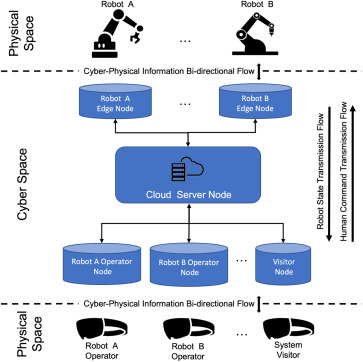
\includegraphics[width=0.5\linewidth]{figs/framework.jpg}
        \caption{The Architecture of Multi-robot Multi-client Communication Mechanism \cite{LI2022102321}}
        \label{f:system-framework}
    \end{figure}

    During information transmission, the control communication flow between each robot and client is encrypted using a hash table. Moreover, in manufacturing practice, the system utilizes commercial cloud servers and employs Secure Sockets Layer \ac{SSL} and \ac{SSTP} encryption methods to ensure system stability and security.

    To implement the concept of a multi-robot collaborative manufacturing system with human-in-the-loop control, a \ac{DT} of the physical robot is modeled using the Unity game engine. The robot twin is then ported to \ac{AR} glasses to enhance the immersive experience, providing both a teleoperation method and a more user-friendly observation approach for the robot. In the \ac{AR} glasses, the \ac{DT} of the robot, synchronized with the real robot, is projected as a hologram in the remote workspace. With the mapped \ac{DT} of the physical robot, remote control of the robot's movement is possible, while its state can be monitored and visualized via the robot \ac{DT}. By integrating the proposed communication mechanism and multiple \ac{AR} teleoperation systems, users can collaborate even when distributed across different locations, aligning with the collaborative manufacturing paradigm.

    The process of transferring the pose of the \ac{DT} to the physical robot, known as registration, consists mainly of two stages: displayed model alignment and joint alignment. In the model alignment stage, using the pre-designed virtual 3D robot model, the Vuforia Engine is employed to align the model targets between the physical and virtual robots, synchronizing the displayed robot pose. Joint value alignment then involves calculating a joint-value transformation matrix based on the pose-aligned models, converting the \ac{DT}'s joint values in the \ac{AR} coordinate system to the physical robot's joint values in the real-world coordinate system.


    Overall, a robot control method aided by \ac{AR} technology offers clear advantages over direct robot control, such as:
    \begin{itemize}
        \item Predictability for the final posture and motion trajectories of the physical robot.
        \item Visualization of trajectories to prevent potential safety issues.
        \item User-friendly interface, allowing the manufacturing system to be manipulated without spatial or human limitations.
    \end{itemize}

    Apart from controlling the robot, observing the environmental information of the workspace and the robot's state during task execution remains challenging. In the proposed system, IP cameras monitor the workspace, and the video feed is projected to the \ac{AR} glasses via a video streaming server. This setup allows both the status of the robot and the real-time status of the workspace to be presented in the \ac{AR} glasses, enhancing remote monitoring efficiency, as illustrated in figure \ref{f:workspace-visualization}.

    \begin{figure}[!htpb]
        \centering
        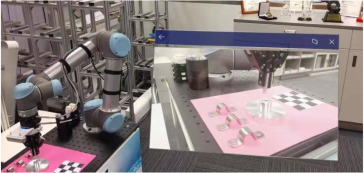
\includegraphics[width=0.7\linewidth]{figs/workspace-visualization.jpg}
        \caption{Demonstration of workspace observation approach \cite{LI2022102321}}
        \label{f:workspace-visualization}   
    \end{figure}
    \FloatBarrier

    Nevertheless, several challenges persist. Networking latency and positioning accuracy are issues presented in the lab-based demonstration. To address networking latency, some novel communication mechanisms (e.g., time-sensitive networks) and technologies (e.g., 5G) are proposed \cite{LI2022102321}. 

% chapter 4 
\section{goal pipeline aligned with the state of the art} % 
After having properly implemented the bidirectional communication between both environments, the on-site and the remote, allowing both members to interact with the robot, the next step was to complement the already built application as well as its interface. 

Afterwards, the framework required to integrate the \ac{MR} technologies with the robotic arm was thoroughly discussed with the supervisors, leading to the following components:
\begin{itemize}
    \item \textbf{On-Site Interaction:}
    \begin{itemize}
        \item Implement an UR10e digital model into the Unity 3D simulation environment
        \item Utilize marker detection, utilizing Vuforia, to align the digital model with the physical robot
        \item Perform pose registration to ensure accurate spatial alignment between the virtual and physical models
        \item Develop a user-friendly interface for robot manipulation using \ac{HHDs}
        \item Implement visual and audio cues for user awareness and accident prevention 
    \end{itemize}
    \item \textbf{Remote Visualization and Interaction:}
    \begin{itemize}
        \item Enable bilateral communication between the robot and the Unity digital twin
        \item Provide remote participants with a foundational 2D interface, such as a laptop screen, to visualize the collaboration scenario and 
        task context.
        \item Implement real-time updates of the robot's position and workspace visualization
        \item Develop the capability for remote operation of the robot via the \ac{MR} application, enhancing the remote participant's ability to 
        interact and manipulate the collaborative environment.
    \end{itemize}
    \item \textbf{Automation and Immersion:}
    \begin{itemize}
        \item Integrate a camera into the robot and develop a camera feed transmission to provide real-time updates of the robot's position and workspace visualization
        \item Share this information with remote participants, assisting on-site participants by delegating visual sharing to the robot.
    \end{itemize}
\end{itemize}



% chapter 4 - this is already discussed - previous text - is it still useful?
% previously was a chapter - re-define its order in the document
\section{Remote Collaboration}
% \label{chapter:remote}
% \begin{introduction}
% The development of the remote member's application will be thoroughly explained in this chapter.
% \end{introduction}



    Building on the foundation of the application that facilitated on-site member interactions, the next critical step was to establish a robust connection to the UR10e robot. This connection was essential for accurately developing a digital twin of the robotic arm, allowing for real-time manipulation and visualization within a Unity environment.

    To achieve this, it was necessary to extend the initial project by developing a complementary application focused on the remote manipulation 
    of the robotic arm through Unity. 

    This bridge facilitated communication between the ROS environment on Ubuntu and the Unity application on Windows, enabling real-time visualization 
    and control of the robot within Unity.

    However, this integration posed significant challenges. Despite the potential of the ROS-TCP-Connector, the documentation provided limited guidance 
    on adapting the connection to different robots beyond the examples in the online tutorial. As a result, the development process relied heavily on 
    trial and error, requiring iterative testing and debugging to achieve a functional ROS-Unity connection.

    

    
    %%%%%%%%%%%%%%%%%%%%%%%%%%%%%%%%%%%%%%%%%%%%%%%%%%%%%%%%%
    do below here - add photos or video that mimic the process, same images
    